% =============================================================================
%  PhD thesis — book-format template
%  170 x 240 mm trim + 3 mm bleed. Compile with pdfLaTeX + BibTeX:
%      latexmk -pdf book.tex
%  Personal details:   thesisinfo.tex
%  Layout and styling: bookformat.tex (book) on top of preamble.tex (packages)
% =============================================================================
\documentclass[
english,
twoside,
openright
]{thesisbook}

% preamble.tex — packages and the chapter front-matter macros (\basedon, \chapterauthors,
% chapterabstract). bookformat.tex restyles them for the printed book.
\usepackage[T1]{fontenc}
\usepackage[utf8]{inputenc}

\usepackage{graphicx}
\usepackage{amsmath, amssymb, mathtools}
%\usepackage{natbib}
\usepackage[authoryear,round]{natbib}
%\usepackage[numbers,sort&compress]{natbib}
\usepackage{setspace}
\usepackage{booktabs}
\usepackage{longtable}
\usepackage{float}
\usepackage{caption}
\usepackage{placeins}
\usepackage{comment}
\usepackage{titlesec}
\usepackage{pdflscape}
\usepackage{xcolor}
\usepackage{csquotes}
\usepackage{ragged2e}
\usepackage{changepage}
\usepackage{textcomp}
\usepackage{marvosym}
\usepackage{array}
\usepackage{microtype}
\usepackage{lastpage}
\usepackage{epstopdf}
\usepackage{bm}
\usepackage{url}
\usepackage{xurl}
\usepackage{breakurl}
\usepackage{subcaption}
\usepackage{tabularx}
\usepackage{tcolorbox}
\usepackage{adjustbox}
\IfFileExists{opensans.sty}{\usepackage{opensans}}{}
\captionsetup[table]{position=bottom}

\captionsetup{width=0.85\textwidth}

\onehalfspacing

\titlespacing*{\section}
{0pt}{2.0ex plus 0.5ex minus 0.2ex}{1.0ex plus 0.2ex}

\titlespacing*{\subsection}
{0pt}{1.6ex plus 0.4ex minus 0.2ex}{0.8ex plus 0.2ex}

\titlespacing*{\subsubsection}
{0pt}{1.2ex plus 0.3ex minus 0.2ex}{0.6ex plus 0.2ex}

\usepackage[hidelinks]{hyperref}

% ---- Chapter front-matter macros (A4 layout; bookformat.tex restyles them for the book) ----
\def\basedonhead{}
\def\basedontext{}
% \basedon[intro line]{citation} — place it directly BEFORE \chapter{...}
\newcommand{\basedon}[2][This chapter is based on:]{\gdef\basedonhead{#1}\gdef\basedontext{#2}}
\newcommand{\chapterauthors}[1]{\begin{center}#1\end{center}}
% \begin{chapterabstract}[Heading] ... \end{chapterabstract}; the heading defaults to "Abstract"
\newenvironment{chapterabstract}[1][Abstract]
  {\if\relax\detokenize{#1}\relax\else\section*{#1}\fi}
  {\par\ifx\basedontext\empty\else\vspace{2em}%
   \begin{tcolorbox}[colback=gray!6,colframe=gray!35,arc=2pt,boxrule=0.4pt,
                     left=8pt,right=8pt,top=6pt,bottom=6pt]
     \small\noindent\textit{\basedonhead}\\[0.3em]\basedontext
   \end{tcolorbox}\gdef\basedontext{}\fi}

% =============================================================================
%  thesisinfo.tex — EVERYTHING PERSONAL LIVES HERE
%  Fill in these fields once; the title page, colophon, running heads and
%  portfolio read them. Leave a field empty, e.g. \newcommand{\ThesisISBN}{},
%  to drop its line from the colophon.
% =============================================================================

% ---------- Title ----------
% The title is set over two lines on the title page.
\newcommand{\ThesisTitleLineOne}{The Main Title of the Thesis}
\newcommand{\ThesisTitleLineTwo}{Continues on a Second Line}
\newcommand{\ThesisSubtitleLineOne}{A Subtitle That Explains}
\newcommand{\ThesisSubtitleLineTwo}{What the Thesis Is About}

% ---------- Author and degree ----------
\newcommand{\ThesisAuthor}{Firstname Lastname}
\newcommand{\ThesisDegree}{Doctoral thesis}
\newcommand{\ThesisInstitution}{Department, University, City}
\newcommand{\ThesisYear}{2026}

% ---------- Supervision (used on the colophon and in the portfolio) ----------
\newcommand{\ThesisSupervisor}{Prof. dr. A.B. Supervisor}
\newcommand{\ThesisCoSupervisor}{Dr. C.D. Co-supervisor}

% ---------- Colophon (page 2) ----------
\newcommand{\ThesisCoverDesign}{Cover designer}
\newcommand{\ThesisPrinting}{Printer}
\newcommand{\ThesisISBN}{978-00-0000-000-0}
\newcommand{\ThesisDOI}{10.0000/000000}
% Licence or copyright notice printed at the foot of the colophon
\newcommand{\ThesisLicence}{This work is licensed under a Creative Commons
  Attribution 4.0 International licence (CC BY 4.0),
  \url{https://creativecommons.org/licenses/by/4.0/}.}

% ---------- Running heads ----------
% One short title per numbered chapter, in order (1 = General introduction).
% Shown in grey on right-hand pages. Add or remove \or lines to match your chapters.
\newcommand{\shortchaptertitle}{\ifcase\value{chapter}%
  \or General introduction%
  \or Short Title of Chapter 2%
  \or Short Title of Chapter 3%
  \or Short Title of Chapter 4%
  \or General discussion\fi}

% bookformat.tex — 170 x 240 mm book layout + 3 mm bleed (176 x 246 mm paper),
% a common format for printed PhD theses. To change the trim size, edit \geometry
% and the TrimBox/BleedBox values below (in bp; 1 mm = 2.8346 bp).
% Load it after preamble.tex and thesisinfo.tex.
% BLEED VERSION: 3 mm bleed on every side. The paper is 176 x 246 mm; the final
% trimmed page (170 x 240 mm) sits centred, so all margins are 3 mm larger.
\geometry{papersize={176mm,246mm}, inner=23mm, outer=23mm,
	top=28mm, bottom=19mm, includefoot=false,
	headheight=12pt, headsep=11mm, footskip=0pt}

% Fonts (all SIL Open Font License): body text in Libertinus Serif 10.5 pt on 14 pt,
% equations in Libertinus Math, headings, running heads, tabs and captions labels in Carlito.
\usepackage{pdfpages}
\pdfpageattr{/TrimBox [8.504 8.504 490.394 688.819] /BleedBox [0 0 498.898 697.323]}
\usepackage{libertinus}% Libertinus Serif (text)
\usepackage[lining]{carlito}% Carlito (sans: headings, running heads, tabs)
\usepackage{libertinust1math}% Libertinus Math (equations)
\renewcommand*{\familydefault}{\rmdefault}\normalfont
\setlength{\emergencystretch}{2em}% lets TeX loosen a line slightly instead of overrunning the margin
\setlength{\intextsep}{10pt}% space above and below [H] figures
\makeatletter\g@addto@macro\@floatboxreset{\def\@tempa{table}\ifx\@captype\@tempa\small\fi}\makeatother% tables one size smaller than the text
\renewcommand{\textsc}[1]{#1}% the class maps \textsc to a weight Libertinus lacks; print the text as written
\renewcommand{\normalsize}{\fontsize{10.5}{14}\selectfont}
\singlespacing\normalsize
\setlength{\parindent}{0pt}
\setlength{\parskip}{14pt}

% Headings
\definecolor{chaptertan}{cmyk}{0,0.30,0.60,0.21}
\definecolor{abstractgrey}{RGB}{220,221,222}% background of the abstract pages
\titleformat{\section}{\sffamily\fontsize{12}{14}\bfseries\color{black}}{\thesection}{0.5em}{}
\titleformat{\subsection}{\sffamily\fontsize{11}{14}\bfseries\color{black}}{\thesubsection}{0.5em}{}
\titleformat{\subsubsection}{\sffamily\fontsize{11}{14}\bfseries\itshape}{}{0pt}{}
\titlespacing*{\section}{0pt}{14pt}{-14pt}
\titlespacing*{\subsection}{0pt}{0pt}{-14pt}
\titlespacing*{\subsubsection}{0pt}{0pt}{-14pt}

% Chapter opener on its own right-hand page, with the "This chapter is based on" note
\definecolor{basedonrule}{cmyk}{0.77,0.37,0.30,0}
\newcommand{\printbasedon}{%
  \ifx\basedontext\empty\else
    \par\vspace{42mm}%
    \noindent\begin{minipage}{\textwidth}\setlength{\parskip}{0pt}%
      {\color{basedonrule}\rule{\textwidth}{1.5pt}}\par\vspace{3pt}%
      \sffamily\fontsize{9.5}{14}\selectfont\raggedleft
      {\bfseries\basedonhead}\par
      \mdseries\basedontext
    \end{minipage}%
    \gdef\basedontext{}%
  \fi}
\titleformat{\chapter}[display]
  {\thispagestyle{empty}\raggedleft\sffamily}
  {\fontsize{54}{60}\bfseries\color{chaptertan}\chaptertitlename~\thechapter}
  {8mm}{\fontsize{14}{18}\bfseries\color{black}}[\printbasedon\clearpage]

% In the book the author block is dropped and the abstract sits on a grey page
\renewcommand{\chapterauthors}[1]{}
\renewenvironment{chapterabstract}[1][Abstract]
  {\clearpage\ifodd\value{page}\thispagestyle{empty}\null\clearpage\fi% reach a left-hand page
   \pagecolor{abstractgrey}\thispagestyle{empty}\null\clearpage% grey left page facing the abstract
   \thispagestyle{empty}\enlargethispage{2\baselineskip}%
   \if\relax\detokenize{#1}\relax\vspace*{0pt}\else\section*{#1}\vspace{14pt}\fi\setlength{\parskip}{6pt}\fontsize{10}{13.5}\selectfont}% abstracts slightly smaller so each fits on one page
  {\par\clearpage\nopagecolor\cleardoublepage}

% Unnumbered chapters (Acknowledgements, Prologue, appendices): title at the top, text follows
\titleformat{name=\chapter,numberless}[block]
  {\raggedright\sffamily\fontsize{14}{18}\bfseries\color{black}}{}{0pt}{}
\titlespacing*{\chapter}{0pt}{45mm}{0pt}
\titlespacing*{name=\chapter,numberless}{0pt}{-8mm}{4pt}

% Running heads at the top, grey: "30 | Chapter 1" (left pages), "Short title | 31" (right pages)
\setlength{\headwidth}{\textwidth}
\fancyhf{}
\renewcommand{\headrulewidth}{0pt}
% \shortchaptertitle (the right-hand running head) is defined in thesisinfo.tex
\newcommand{\evenheadtext}{\ifnum\value{chapter}>0 Chapter~\thechapter\fi}
\newcommand{\oddheadtext}{\shortchaptertitle}
\fancyhead[LE]{\sffamily\color{gray}{\fontsize{9}{9}\selectfont\thepage}%
  \hspace{0.5em}\textbar\hspace{0.5em}{\fontsize{8}{9}\selectfont\evenheadtext}}
\fancyhead[RO]{\sffamily\color{gray}{\fontsize{8}{9}\selectfont\oddheadtext}%
  \hspace{0.5em}\textbar\hspace{0.5em}{\fontsize{9}{9}\selectfont\thepage}}
\fancypagestyle{plain}{\fancyhf{}\renewcommand{\headrulewidth}{0pt}}
\let\oldappendix\appendix
\renewcommand{\appendix}{\oldappendix
  \renewcommand{\evenheadtext}{Appendices}\renewcommand{\oddheadtext}{Appendices}%
  % appendix headings: larger, with a blank line before the text
  \titleformat{\section}{\sffamily\fontsize{14}{18}\bfseries\color{black}}{\thesection}{0.5em}{}%
  \titlespacing*{\section}{0pt}{0pt}{0pt}%
  \titleformat{\subsection}{\sffamily\fontsize{11}{14}\bfseries\color{black}}{\thesubsection}{0.5em}{}%
  \titlespacing*{\subsection}{0pt}{0pt}{-6pt}}

% Contents heading in the same style as other front-matter headings
\renewcommand{\cfttoctitlefont}{\sffamily\fontsize{14}{18}\selectfont\bfseries\color{black}}

% Captions and bibliography
\captionsetup{font={small,color=black}, labelfont={bf,sf}, labelsep=period, width=\textwidth}
\renewcommand{\bibfont}{\fontsize{8}{10.5}\selectfont}
% URLs in the text font
\urlstyle{same}

% Chapter thumb tabs on right-hand pages (tan tab at the page edge, stepping down per chapter).
% Each tab is 16.3 mm tall, so about 12 tabs (chapters + appendix) fit down the page edge.
\newcommand{\thumblabel}{\arabic{chapter}}
\newcommand{\thumbindex}{\value{chapter}}
\newif\ifthumbtab
\newcommand{\thumbtab}{%
  \ifnum\value{chapter}>0 \thumbtabtrue\fi
  \ifthumbtab
  \begin{tikzpicture}[remember picture,overlay]
    \pgfmathsetlengthmacro{\thumbtop}{-24.9mm-16.3mm*(\thumbindex-1)}
    \fill[chaptertan,rounded corners=1.2mm]
      ([xshift=-16.7mm,yshift=\thumbtop-3mm]current page.north east) rectangle ++(17mm,-16.3mm);% 13.7 mm visible after trimming
    \node[text=white,font=\sffamily\fontsize{12}{12}\selectfont\bfseries]
      at ([xshift=-11.35mm,yshift=\thumbtop-11.15mm]current page.north east) {\thumblabel};
  \end{tikzpicture}%
  \fi}
\fancyhead[RO]{\thumbtab\sffamily\color{gray}{\fontsize{8}{9}\selectfont\oddheadtext}%
  \hspace{0.5em}\textbar\hspace{0.5em}{\fontsize{9}{9}\selectfont\thepage}}
\let\oldappendixthumb\appendix
\renewcommand{\appendix}{% the appendix tab sits one step below the last chapter's tab
  \edef\thumbindex{\the\numexpr\value{chapter}+1\relax}\oldappendixthumb
  \thumbtabtrue\renewcommand{\thumblabel}{A}}

% No running head or tab on blank left-hand pages before a chapter opener
\usepackage{emptypage}

% Paragraph headings (e.g. "Perturbation waveforms."): black italic on their own line, as in the proof
\titleformat{\paragraph}[block]{\fontsize{11}{14}\itshape\color{black}}{}{0pt}{}
\titlespacing*{\paragraph}{0pt}{0pt}{-14pt}
\titleformat{\subparagraph}[block]{\fontsize{10.5}{14}\itshape\color{black}}{}{0pt}{}
\titlespacing*{\subparagraph}{0pt}{0pt}{-14pt}

% Black list markers, numbers and contents entries (the class sets them in red)
\renewcommand*\labelitemi{\textbullet}
\renewcommand*\labelitemii{--}
\renewcommand*\labelitemiii{$\diamond$}
\renewcommand*\labelitemiv{\textperiodcentered}
\renewcommand{\labelenumi}{\arabic{enumi}.}
\renewcommand{\labelenumii}{\arabic{enumi}.\arabic{enumii}.}
\renewcommand{\labelenumiii}{\arabic{enumi}.\arabic{enumii}.\arabic{enumiii}.}
\renewcommand{\labelenumiv}{\arabic{enumi}.\arabic{enumii}.\arabic{enumiii}.\arabic{enumiv}.}
\renewcommand{\cftchapfont}{\bfseries\color{black}}

% ---------- Chapter artwork ----------
% openers/Chapterpage.pdf (your designer's chapter artwork, 180 x 250 mm including 5 mm bleed;
% a plain placeholder is supplied — delete or replace it; without the file no artwork page is added)
% is placed at full size on a right-hand page before each numbered chapter opener,
% with a page in the artwork's background colour on its back, and the chapter number is printed on top of it.
% Set artworkback to the background colour of your own artwork.
% Number: Carlito Bold 122 pt, CMYK 0/30/60/21, at the position used in the
% original design. Switched off in the appendices; add \chapterart{A} after \appendix in book.tex if you want an artwork page there too.
\newlength{\artbleed}\setlength{\artbleed}{3mm}% distance from paper edge to trim edge
\definecolor{chapternumtan}{cmyk}{0,0.30,0.60,0.21}
\definecolor{artworkback}{cmyk}{0,0.02,0.06,0.04}% background of the artwork (light warm grey), used for its back page
\newif\ifchapterart \chapterarttrue
\newcommand{\chapterart}[1]{%
  \clearpage\ifodd\value{page}\thispagestyle{empty}\null\clearpage\fi% reach a left-hand page
  \IfFileExists{openers/Chapterpage.pdf}{%
    \pagecolor{artworkback}\thispagestyle{empty}\null\clearpage% coloured left page facing the artwork
    \thispagestyle{empty}\null
    \begin{tikzpicture}[remember picture,overlay]
      \node[inner sep=0pt,outer sep=0pt] at (current page.center)
        {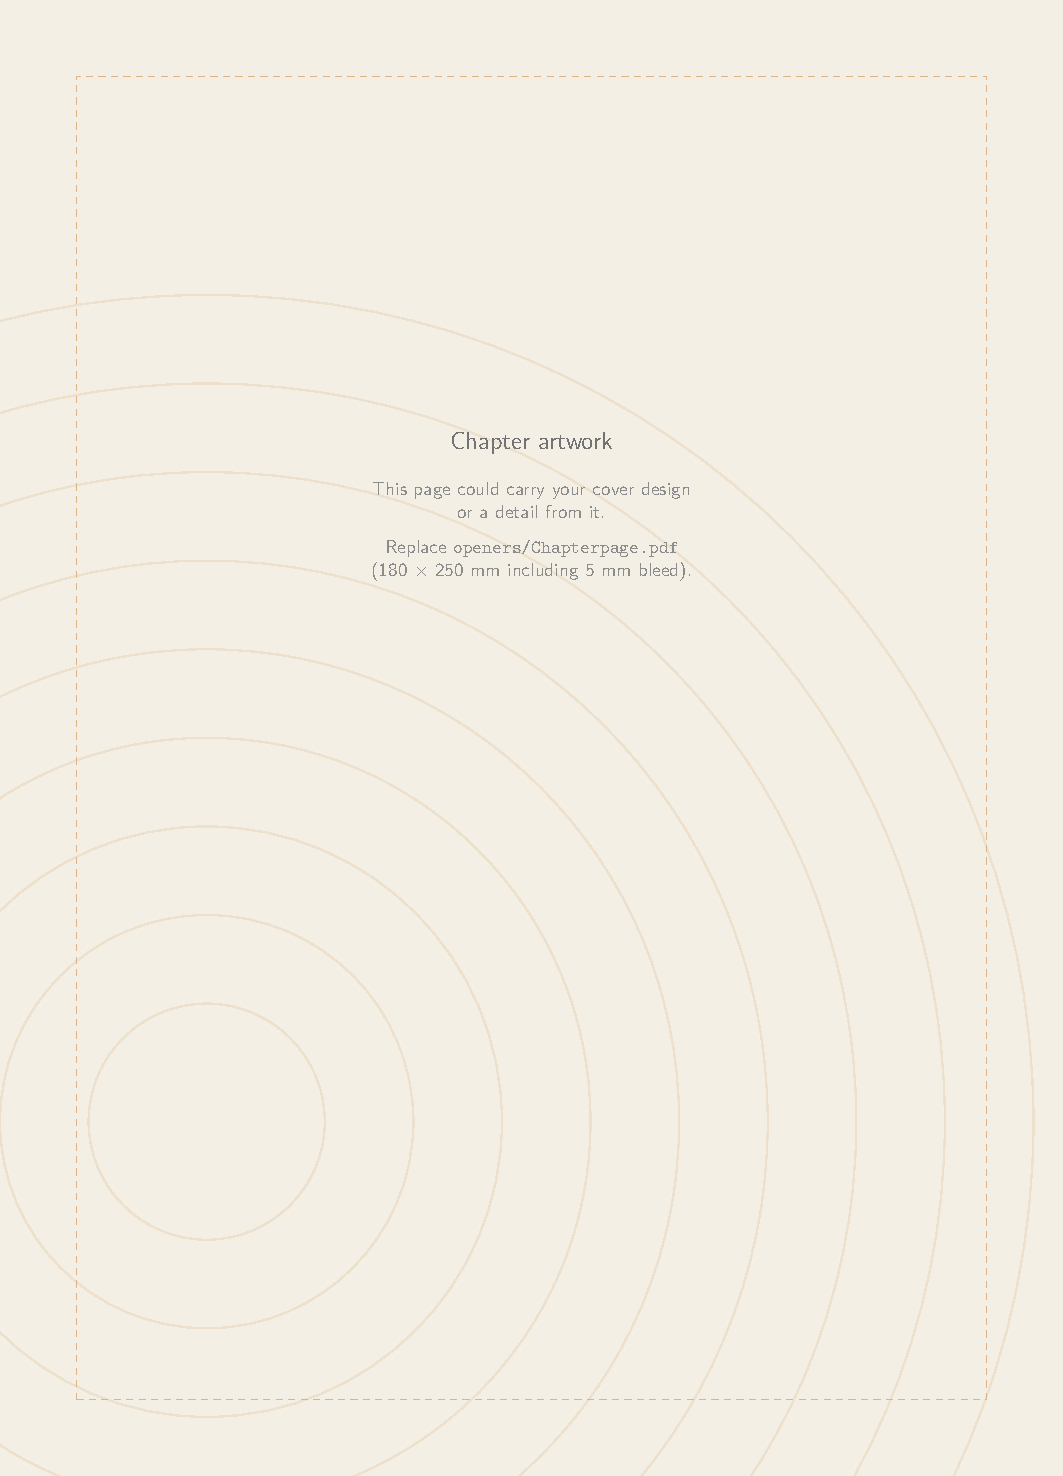
\includegraphics{openers/Chapterpage.pdf}};
      \node[anchor=base,inner sep=0pt,outer sep=0pt,text=chapternumtan]
        at ([xshift=341.58bp+\artbleed,yshift=-550.03bp-\artbleed]current page.north west)
        {\sffamily\fontsize{122bp}{122bp}\selectfont\bfseries #1};
    \end{tikzpicture}%
    \clearpage\nopagecolor\cleardoublepage}{\cleardoublepage}}
\makeatletter
\let\bookorigchapter\chapter
\renewcommand{\chapter}{\@ifstar{\bookorigchapter*}%
  {\ifchapterart\chapterart{\the\numexpr\value{chapter}+1\relax}\fi\bookorigchapter}}
\makeatother
\let\oldappendixart\appendix
\renewcommand{\appendix}{\oldappendixart\chapterartfalse}



\begin{document}

	% ---------- Front matter ----------
	\pagenumbering{arabic}
	% Title page (page 1) and colophon (page 2). All text comes from thesisinfo.tex.
% Positions are measured from the top of the trimmed page (3 mm inside the bleed).
\begingroup\pagestyle{empty}\sffamily% title page and colophon in Carlito
\definecolor{tptan}{cmyk}{0,0.30,0.60,0.21}

% ---------- page 1: title page ----------
\clearpage\thispagestyle{empty}\null
\begin{tikzpicture}[remember picture,overlay]
  \node[anchor=base,inner sep=0pt] at ([yshift=-98mm-3mm]current page.north)
    {\fontsize{15}{15}\selectfont\textls[140]{\MakeUppercase{\ThesisTitleLineOne}}};
  \node[anchor=base,inner sep=0pt] at ([yshift=-106.5mm-3mm]current page.north)
    {\fontsize{15}{15}\selectfont\textls[140]{\MakeUppercase{\ThesisTitleLineTwo}}};
  \draw[tptan,line width=0.5pt] ([xshift=-9mm,yshift=-114mm-3mm]current page.north)
    -- ([xshift=9mm,yshift=-114mm-3mm]current page.north);
  \node[anchor=base,inner sep=0pt] at ([yshift=-123mm-3mm]current page.north)
    {\fontsize{10.5}{10.5}\selectfont\itshape \ThesisSubtitleLineOne};
  \node[anchor=base,inner sep=0pt] at ([yshift=-128.5mm-3mm]current page.north)
    {\fontsize{10.5}{10.5}\selectfont\itshape \ThesisSubtitleLineTwo};
  \node[anchor=base,inner sep=0pt] at ([yshift=-200mm-3mm]current page.north)
    {\fontsize{9.5}{9.5}\selectfont\textls[160]{\MakeUppercase{\ThesisAuthor}}};
  \node[anchor=north,inner sep=0pt,align=center,text=gray,font=\fontsize{8}{11}\selectfont]
    at ([yshift=-205mm-3mm]current page.north) {\ThesisDegree\\\ThesisInstitution\\\ThesisYear};
\end{tikzpicture}

% ---------- page 2: colophon ----------
\clearpage\thispagestyle{empty}
\newcommand{\colline}[2]{\if\relax\detokenize{#2}\relax\else#1: #2\par\fi}
\vspace*{\fill}
{\fontsize{8.5}{12}\selectfont\setlength{\parskip}{0pt}\raggedright
  {\bfseries \ThesisAuthor}\par
  {\bfseries \ThesisTitleLineOne{} \ThesisTitleLineTwo}\par
  {\itshape \ThesisSubtitleLineOne{} \ThesisSubtitleLineTwo}\par
  \medskip
  \colline{Supervisor}{\ThesisSupervisor}
  \colline{Co-supervisor}{\ThesisCoSupervisor}
  \medskip
%  \colline{Cover design}{\ThesisCoverDesign}
%  \colline{Printing}{\ThesisPrinting}
%  \colline{ISBN}{\ThesisISBN}
%  \colline{DOI}{\ThesisDOI}
%  \medskip
%  \ThesisLicence\par}
%\clearpage\endgroup
        % pages 1-2: title page and colophon
	\tableofcontents
	\clearpage

	\clearpage
\chapter*{Acknowledgements}
\addcontentsline{toc}{chapter}{Acknowledgements}

% Write your acknowledgements here. Use \newpage to control where a page breaks.


	\clearpage
\chapter*{Prologue}
\addcontentsline{toc}{chapter}{Prologue}

% Optional: a short personal prologue. Delete this file and its \input line in
% book.tex if you do not want one.

\begingroup
\setlength{\parindent}{0pt}
\setlength{\parskip}{0.9em}
\linespread{1.08}\selectfont

[Opening paragraph of the prologue.]

[Second paragraph.]

\begin{center}
	\emph{[A centred line set apart from the text.]}
\end{center}

[Further paragraphs.]

\begin{flushright}
	\emph{[A closing line, set flush right.]}
\end{flushright}

\endgroup


	% ---------- Main matter ----------
	% Each numbered chapter gets an artwork page, an opener, and a grey abstract
	% spread automatically. Add or remove chapters here and update
	% \shortchaptertitle in thesisinfo.tex to match.
	% General introduction (Chapter 1). No \basedon: it is not based on a paper.
\chapter{General Introduction}

% chapterabstract with an empty heading: the text sits on the grey spread
% without an "Abstract" title. Use it for an opening passage.
\begin{chapterabstract}[]
[An opening passage for the thesis. It is set on its own page, facing a grey left-hand page.]

[A second paragraph.]
\end{chapterabstract}

\section{First Section of the Introduction}
[Introductory text. Cite with \verb|\citep| or \verb|\citet|: e.g. \citep{placeholderArticle2024} or \citet{placeholderBook2020}.]

\begin{figure}[htbp]
	\centering
	\includegraphics[width=\textwidth]{figures/placeholder.pdf}
	\caption{\textbf{Figure title.} Caption text. Figures shared by the introduction and discussion live in \texttt{figures/}.}
	\label{fig:intro-placeholder}
\end{figure}

\subsection{A Subsection}
[Text. Equations are numbered per chapter:]
\begin{equation}
	\frac{dz}{dt} = (a + i\omega)\,z - |z|^2 z .
	\label{eq:intro-example}
\end{equation}

\subsection{Another Subsection}
[Text referring to Figure~\ref{fig:intro-placeholder} and Equation~\ref{eq:intro-example}.]

\section{Second Section of the Introduction}
[Text.]

\section{Thesis Overview}
[Chapter~2 \ldots]

[Chapter~3 \ldots]

[Chapter~4 \ldots]

[Finally, Chapter~5 synthesises \ldots]

	% ---------------------------------------------------------------------------
% Chapter based on a PUBLISHED paper.
% \basedon goes directly BEFORE \chapter: it prints the citation on the opener.
% \chapterauthors is kept for the A4 version but hidden in the book layout.
% \chapterabstract puts the abstract on its own page, facing a grey page.
% ---------------------------------------------------------------------------
\basedon[This chapter is based on:]{%
Lastname F.$^{*}$, Coauthor A.$^{*}$, and Coauthor B. (2025). Title of the published paper. \textit{Journal Name}, 1, 100. \url{https://doi.org/10.0000/example}}
\chapter{Full Title of the First Research Chapter, as Published}
\renewcommand{\thefigure}{\thechapter.\arabic{figure}}
\setcounter{figure}{0}

\chapterauthors{%
	Firstname Lastname$^{*}$, Author Two$^{*}$, Author Three$^{\dagger}$

	\vspace{0.5em}

	Department, University, City, Country

	\vspace{0.5em}

	\small
	$^{*}$Shared first authors.\\
	$^{\dagger}$Corresponding author: Author Three (\texttt{email@example.org})
}

\begin{chapterabstract}
[Abstract of the paper, as published.]
\end{chapterabstract}

\section{Introduction}
[Text \citep{placeholderArticle2024}.]

\section{Methods}
\subsection{Participants}
[Text.]

\paragraph{A paragraph heading.}
[Paragraph headings sit on their own line in italics.]

\subsection{Analysis}
[Text. Table~\ref{tab:ch2-example} shows a booktabs table.]

\begin{table}[htbp]
	\centering
	\caption{\textbf{Table title.} Caption text.}
	\label{tab:ch2-example}
	\begin{tabular}{@{}lcc@{}}
		\toprule
		\textbf{Measure} & \textbf{Group A} & \textbf{Group B} \\
		\midrule
		Measure 1 & 0.00 & 0.00 \\
		Measure 2 & 0.00 & 0.00 \\
		\bottomrule
	\end{tabular}
\end{table}

\section{Results}
[Text referring to Figure~\ref{fig:ch2-placeholder}.]

\begin{figure}[htbp]
	\centering
	\includegraphics[width=0.9\linewidth]{chapters/chapter1/figures/placeholder.pdf}
	\caption{\textbf{Figure title.} Caption text. Keep each chapter's figures in its own \texttt{figures/} folder.}
	\label{fig:ch2-placeholder}
\end{figure}

\section{Discussion}
[Text.]

\section{Conclusion}
[Text.]

\section{Acknowledgements}
[Funding statement.]

	% ---------------------------------------------------------------------------
% Chapter based on a PREPRINT, with a graphical abstract and a supplement.
% The optional argument of \basedon replaces "This chapter is based on:".
% ---------------------------------------------------------------------------
\basedon[This chapter is based on a manuscript currently under journal consideration. A preprint is available as:]{%
Lastname F., Coauthor A., and Coauthor B. Title of the preprint. \textit{bioRxiv} 2025. \url{https://doi.org/10.0000/example}}
\chapter{Full Title of the Second Research Chapter}
\renewcommand{\thefigure}{\thechapter.\arabic{figure}}
\setcounter{figure}{0}

\chapterauthors{%
	Firstname Lastname, Author Two, Author Three$^{*}$

	\vspace{0.5em}

	Department, University, City, Country

	\vspace{0.5em}

	\small
	$^{*}$Corresponding author: \texttt{email@example.org}
}

\begin{chapterabstract}
[Abstract text.]
\vspace{0.5em}
% Optional graphical abstract on the abstract page
\begin{figure}[htbp]
	\centering
	\includegraphics[width=\textwidth]{chapters/chapter2/figures/placeholder.pdf}
	\caption*{}
\end{figure}
\end{chapterabstract}

\section{Introduction}
[Text \citep{placeholderArticle2024, placeholderPreprint2025}.]

\section{Methods}
\subsection{Model}
[Text.]

\section{Results}
\subsection{First Result}
[Text referring to Figure~\ref{fig:ch3-main} and Supplementary Figure~\ref{fig:ch3-supp}.]

\begin{figure}[htbp]
	\centering
	\includegraphics[width=\linewidth]{chapters/chapter2/figures/placeholder.pdf}
	\caption{\textbf{Figure title.} Caption text.}
	\label{fig:ch3-main}
\end{figure}

\section{Discussion}
\subsection{Limitations and future directions}
[Text.]

\section{Acknowledgements}
[Funding statement.]

% ---------- Supplementary material: figures numbered S1, S2, ... ----------
\clearpage
\renewcommand{\thefigure}{S\arabic{figure}}
\renewcommand{\thetable}{S\arabic{table}}
\setcounter{figure}{0}
\setcounter{table}{0}
\section{Supplementary Material}
\subsection{Supplementary analysis}
[Text.]

\begin{figure}[htbp]
	\centering
	\includegraphics[width=0.85\textwidth]{chapters/chapter2/figures/placeholder.pdf}
	\caption{\textbf{Supplementary figure title.} Caption text.}
	\label{fig:ch3-supp}
\end{figure}

% Restore chapter numbering for the following chapters
\renewcommand{\thefigure}{\thechapter.\arabic{figure}}
\renewcommand{\thetable}{\thechapter.\arabic{table}}

	% ---------------------------------------------------------------------------
% Chapter based on a manuscript IN PREPARATION, with a structured abstract
% and a long supplementary table that breaks across pages (longtable).
% ---------------------------------------------------------------------------
\basedon{%
Firstname Lastname, Author Two, Author Three (2026). \textit{Title of the manuscript.} In preparation.}
\chapter{Full Title of the Third Research Chapter}
\setcounter{figure}{0}
\renewcommand{\thefigure}{\thechapter.\arabic{figure}}

\chapterauthors{%
	Firstname Lastname$^{1,*}$, Author Two$^{2}$, Author Three$^{1}$

	\vspace{0.5em}

	$^{1}$Department, University, City, Country

	\vspace{0.25em}

	$^{2}$Second affiliation

	\vspace{0.5em}

	\small
	$^{*}$Corresponding author: \texttt{email@example.org}
}

\begin{chapterabstract}
\noindent\textbf{Background.}
[Text.]

\noindent\textbf{Objective.}
[Text.]

\noindent\textbf{Methods.}
[Text.]

\noindent\textbf{Results.}
[Text.]

\noindent\textbf{Conclusions.}
[Text.]
\end{chapterabstract}

\section{Introduction}
[Text \citep{placeholderArticle2024}.]

\section{Methods}
\subsection{Study overview}
[Text. Protocol parameters are listed in Table~\ref{tab:ch4-long}.]

\section{Results}
[Text referring to Figure~\ref{fig:ch4-main}.]

\begin{figure}[htbp]
	\centering
	\includegraphics[width=0.8\linewidth]{chapters/chapter3/figures/placeholder.pdf}
	\caption{\textbf{Figure title.} Caption text.}
	\label{fig:ch4-main}
\end{figure}

\section{Discussion}
[Text.]

\section*{Declaration of competing interest}
[Statement.]

\section*{Data availability}
[Statement.]

\section*{Acknowledgements}
[Funding statement.]

% ---------- Supplementary material ----------
\clearpage
\renewcommand{\thefigure}{S\arabic{figure}}
\renewcommand{\thetable}{S\arabic{table}}
\setcounter{figure}{0}
\setcounter{table}{0}
\section{Supplementary}
\subsection{Parameter table}

{\fontsize{8}{10.5}\selectfont
\setlength{\tabcolsep}{3pt}\renewcommand{\arraystretch}{1.25}
\begin{longtable}{@{}>{\raggedright\arraybackslash}p{0.34\linewidth}>{\raggedright\arraybackslash}p{\dimexpr0.66\linewidth-6pt\relax}@{}}
\caption{\textbf{Long table title.} A table that continues across pages.}\label{tab:ch4-long}\\
\toprule
\endfirsthead
\multicolumn{2}{@{}l}{\textit{Table \thetable\ (continued)}}\\
\toprule
\endhead
\bottomrule
\endfoot
\bottomrule
\endlastfoot
	\rowcolor{black!18}\multicolumn{2}{@{}l@{}}{\hspace{3pt}\textbf{Group heading}} \\
	Parameter 1 & Value \\
	Parameter 2 & Value \\
	\rowcolor{black!18}\multicolumn{2}{@{}l@{}}{\hspace{3pt}\textbf{Second group heading}} \\
	Parameter 3 & Value \\
	Parameter 4 & Value \\
\end{longtable}
}

\renewcommand{\thefigure}{\thechapter.\arabic{figure}}

\renewcommand{\thetable}{\thechapter.\arabic{table}}

	\chapter{General Discussion}
\renewcommand{\thefigure}{\thechapter.\arabic{figure}}
\setcounter{figure}{0}

% Optional opening passage on a grey spread, as in the introduction:
%\begin{chapterabstract}[]
% Text.
%\end{chapterabstract}
\cleardoublepage

\section{Overview and Synthesis}
[Restate the central aim and the principal findings.]

\section{First Theme}
[Text \citep{placeholderBook2020}.]

\begin{figure}[htbp]
	\centering
	\includegraphics[width=0.95\linewidth]{figures/placeholder.pdf}
	\caption{\textbf{Figure title.} Caption text.}
	\label{fig:disc-placeholder}
\end{figure}

\section{Second Theme}
[Text.]

\section{Future Perspectives}
[Text.]

\section{Summary}
[Text.]


	% ---------- Back matter ----------
	% The appendices follow the last chapter on the next right-hand page,
	% under an "A" thumb tab. Remove any you do not need.
	\cleardoublepage
	\appendix
	\phantomsection
	\addcontentsline{toc}{chapter}{Appendices}

	\section*{Summary}
\addcontentsline{toc}{section}{Summary}

% A plain-language summary. Many universities also ask for a summary in the
% national language: copy this file, change the heading (e.g. "Samenvatting",
% "Zusammenfassung") and add it to book.tex.

	\clearpage
	\section*{Nederlandse samenvatting}
\addcontentsline{toc}{section}{Nederlandse samenvatting}

% Summary in Dutch (required by Dutch universities). For another language,
% change the heading (e.g. "Zusammenfassung", "Résumé") and rename the file.
  % Dutch summary; rename or remove for other languages
	\clearpage
	\section*{About the Author}
\addcontentsline{toc}{section}{About the Author}


	\clearpage
	\section*{Research data management}
\addcontentsline{toc}{section}{Research data management}

% Optional: many universities and funders ask for a research data management
% statement. The headings follow the FAIR principles; replace the bracketed text.

\begingroup

Research Data Management for this thesis was conducted in accordance with the FAIR principles, whenever ethically and legally possible. [Describe the kinds of data in this thesis: newly acquired, previously acquired, public datasets, simulations.]

\textbf{Ethics}

[State the ethical framework, e.g. the Declaration of Helsinki.]

[Per chapter: the approving ethics committee and reference number, and how informed consent was obtained.]

\textbf{Findable and Accessible}

[Where the data and documentation are stored, and who has access.]

[Per chapter: whether and how the data can be accessed, e.g. a repository DOI or ``on reasonable request''.]

[Where the analysis code is archived, e.g. GitHub, Zenodo or an institutional repository.]

\textbf{Interoperable and Reusable}

[File formats and data standards used, e.g. BIDS.]

[Software used and where methodological details are reported.]

\textbf{Privacy}

[How participant privacy was safeguarded: pseudonymisation, storage, GDPR compliance.]

\endgroup

	\clearpage
	% --- colour & helper commands (move to preamble if you reuse elsewhere) ---
\definecolor{pfaccent}{HTML}{30475E}

\newcommand{\pfrule}{%
	\par\noindent{\color{pfaccent!55}\rule{\linewidth}{0.5pt}}\vspace{6pt}\par
}

\newcommand{\pfentry}[4]{%
	% #1 year, #2 title, #3 subtitle (e.g. grant info), #4 description
	\par\noindent
	\begin{minipage}[t]{0.16\textwidth}
		\color{pfaccent}\bfseries #1
	\end{minipage}%
	\begin{minipage}[t]{0.82\textwidth}
		\textbf{#2}\\[1pt]
		{\small\itshape #3}\\[5pt]
		#4
	\end{minipage}
	\par\vspace{10pt}
}

\newcommand{\pfentrysimple}[3]{%
	% #1 year, #2 title, #3 description/context
	\par\noindent
	\begin{minipage}[t]{0.16\textwidth}
		\color{pfaccent}\bfseries #1
	\end{minipage}%
	\begin{minipage}[t]{0.82\textwidth}
		\textbf{#2}\\[2pt]
		{\itshape #3}
	\end{minipage}
	\par\vspace{10pt}
}

\section*{PhD Portfolio}
\addcontentsline{toc}{section}{PhD Portfolio}

\noindent
\begin{tabularx}{\textwidth}{@{}>{\bfseries}l X@{}}
	Name:              & \ThesisAuthor \\[2pt]
	Department:        & [Department or centre] \\[2pt]
	PhD Supervisor:    & \ThesisSupervisor \\[2pt]
	PhD Co-supervisor: & \ThesisCoSupervisor \\[2pt]
	Research Period:   & [Month Year]--[Month Year] \\[2pt]
	PhD Job:           & [Optional: additional role] \\
\end{tabularx}

\vspace{0.1cm}

\subsection*{Research Projects \& Coordination}
\pfrule

% \pfentry{years}{title}{funding / subtitle}{description}
\pfentry{2022--2026}{[Project acronym --- Project name]}{[Funder, Grant No.\ 000000]}{[One-line description of your role in the project.]}

\pfentry{2022--2026}{[Second project]}{[Funder, Grant No.\ 000000]}{[One-line description.]}

\vspace{0.1cm}

\subsection*{Conferences \& Workshops}
\pfrule

\noindent
\begin{tabularx}{\textwidth}{@{}l X l l@{}}
	\toprule
	\textbf{Year} & \textbf{Event} & \textbf{Role} & \textbf{Location} \\
	\midrule
	2026 & [Conference name] & Poster presentation & [City, Country] \\
	2025 & [Workshop name] & Participant & [City, Country] \\
	2024 & [Conference name] & Talk & [City, Country] \\
	\bottomrule
\end{tabularx}

\vspace{0.11cm}
\newpage
\subsection*{Teaching and Mentoring}
\pfrule

% \pfentrysimple{years}{title}{context}
\pfentrysimple{2023--2024}{[Teaching activity]}{[Course or programme]}

\vspace{0.1cm}

\subsection*{Student Supervision}
\pfrule

\noindent
\begin{tabularx}{\textwidth}{@{}X l@{}}
	\toprule
	\textbf{Student} & \textbf{Programme} \\
	\midrule
	{[Student name]} & Master's internship \\
	{[Student name]} & Bachelor's thesis \\
	\bottomrule
\end{tabularx}

	\clearpage
	\section*{List of publications}
\addcontentsline{toc}{section}{List of publications}

\subsection*{Publications included in this thesis}

\begin{tabular}{>{\footnotesize\bfseries}r >{\footnotesize}p{0.85\linewidth}}

	2026 & \textbf{Lastname, F.}, Coauthor, A., \& Coauthor, B. (2026).
	\emph{Title of the first paper}.
	Journal Name, 1, 100.
	\href{https://doi.org/10.0000/example}{doi:10.0000/example}. \\[0.8em]

	2025 & Coauthor, A., \textbf{Lastname, F.}, \& Coauthor, B. (2025).
	\emph{Title of the second paper}.
	bioRxiv.
	\href{https://doi.org/10.0000/example}{doi:10.0000/example}. \\[0.8em]

\end{tabular}

\vspace{1.2em}

\subsection*{Other publications}

\begin{tabular}{>{\footnotesize\bfseries}r >{\footnotesize}p{0.85\linewidth}}

	2024 & \textbf{Lastname, F.}, \& Coauthor, C. (2024).
	\emph{Title of another paper}.
	Journal Name, 2, 200.
	\href{https://doi.org/10.0000/example}{doi:10.0000/example}. \\[0.8em]

\end{tabular}


	\cleardoublepage
	\phantomsection
	\addcontentsline{toc}{section}{Bibliography}
	\renewcommand{\evenheadtext}{Bibliography}\renewcommand{\oddheadtext}{Bibliography}
	\bibliographystyle{apalike-trunc}
	\bibliography{references}

\end{document}
